\chapter{Conceitos Básicos}
\label{ch:2}
Neste capítulo discutiremos alguns conceitos básicos necessários ao entendimento da solução proposta.

\section{Orientação a Servicos}
TODO

\section{Orientação a Componentes}
TODO

\section{Clico PDCA de Desenvolvimento}
TODO

\begin{figure}[htp]
\centering
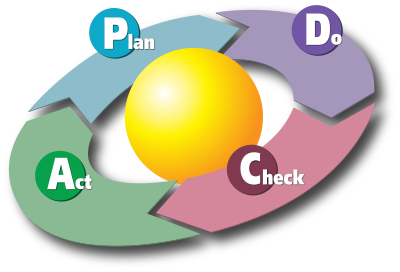
\includegraphics[width=5cm]{chapters/intro/pdca_cycle.png}
\caption[Ciclo PDCA]{Ciclo PDCA de Desenvolvimento com Foco na Melhoria Contínua.}
\label{fig:pdca}
\end{figure}

\section{JMX}
\textit{Java Management Extensions} (JMX) é uma API que fornece uma maneira simples e padrão de gestão e monitoramento de recursos para a plataforma Java. Estes recursos podem ser aplicações, dispositivos, serviços ou a própria JVM (\textit{Java Virtual Machine}). São instrumentados por um ou mais \textit{Managed Beans}, ou simplesmente MBeans, responsáveis por adquirir, manipular ou enviar informações acerca destes recursos~\cite{lindfors2002jmx}.

Essa tecnologia foi desenvolvida através do JCP (\textit{Java Community Process}), em duas JSRs (\textit{Java Specification Request}) distintas. A JSR 3, \textit{Java Management Extensions Instrumentation and Agent Specification} e a JSR 160, \textit{Java Management Extensions Remote API}, ver Seção \ref{subsec:arch}.

JCP é o processo de desenvolvimento padrão de novas especificações para a plataforma Java, as chamadas JRSs. JSRs são documentos que descrevem as especificações e tecnologias propostas à plataforma.

A especificação de JMX define, além da arquitetura, padrões de projeto, API's e um conjunto de serviços de gerenciamento e monitoramento. Possibilitando o desenvolvimento de aplicações gerenciáveis local ou remotamente através do processo de instrumentação, onde atributos, configurações e capacidades da aplicação são expostos. Aumentando a robustez e extensibilidade da aplicação, uma vez que, é possível construir soluções de gerenciamento inteligentes, interoperáveis e independentes da infra-estrutura de gestão~\cite{jmx}.

\subsection{Arquitetura}
\label{subsec:arch}
A arquitetura JMX é definida em três níveis, ver Figura \ref{fig:arch_jmx}:

\begin{itemize}
 \item Nível de Instrumentação;
 \item Nível de Agente;
 \item Nível de Gerenciamento.
\end{itemize}

Como foi dito anteriormente, JMX foi definida segundo duas JSRs , JSR 3 e JSR 160. Os dois primeiros níveis da arquitetura (Instrumentação e Agente) foram definidos na JSR 3, enquanto o Nível de Gerenciamento foi definido na JSR 160. Isso mostra, de certa forma, o potencial de extensibilidade da tecnologia.

\begin{figure}[htp]
\centering
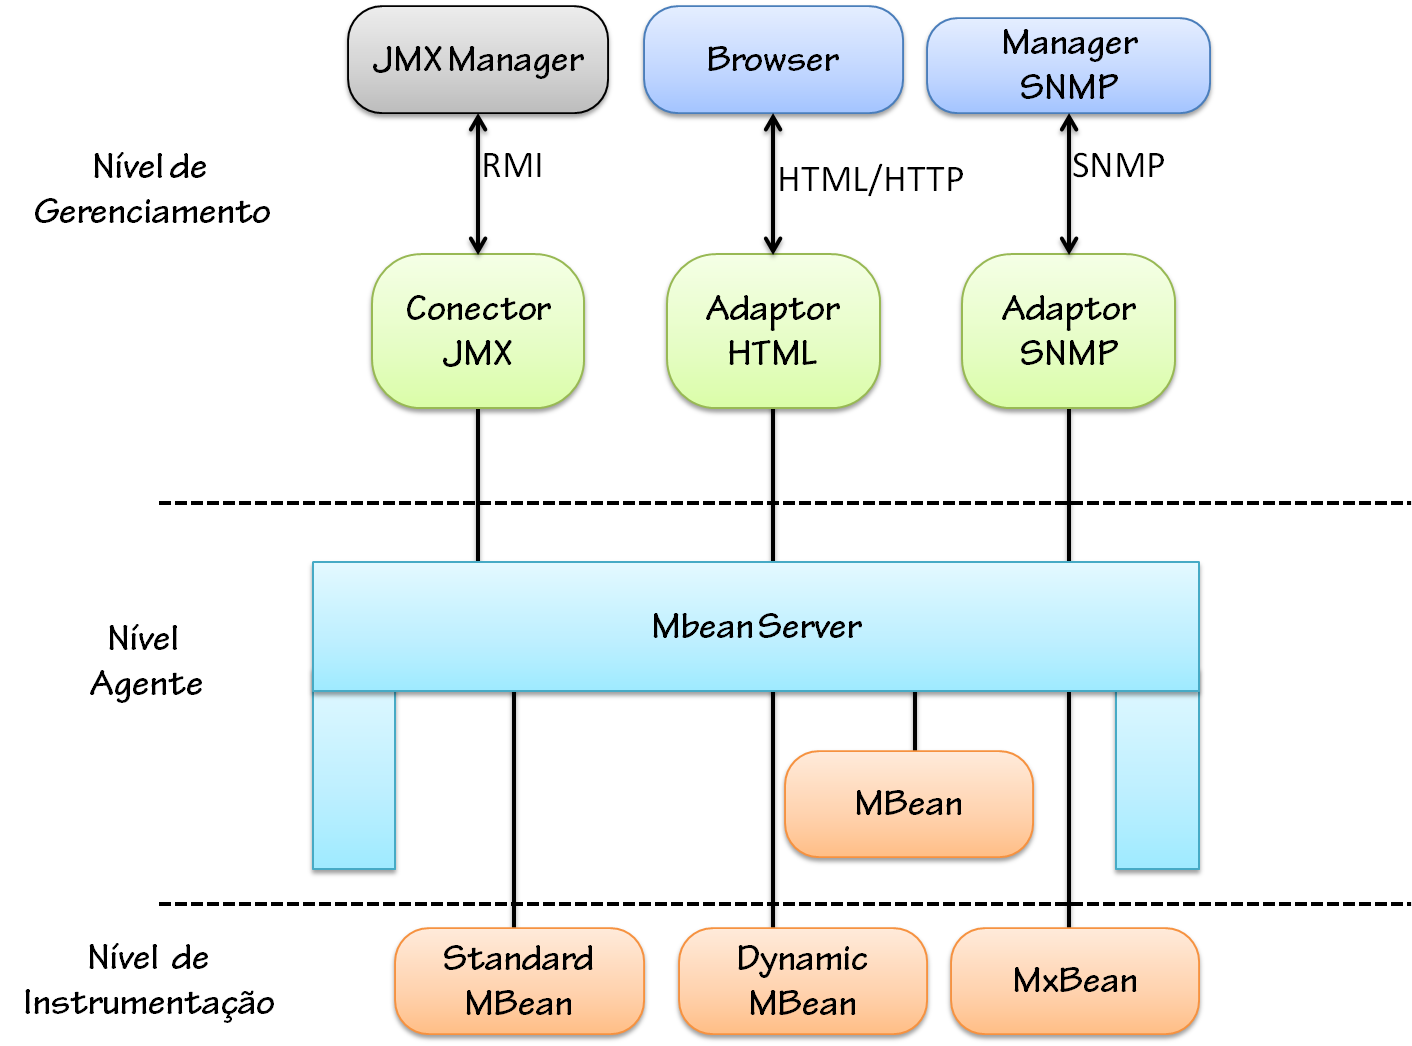
\includegraphics[width=12cm]{chapters/chapter4/arch_jmx.png}
\caption[Arquitetura JMX]{Arquitetura JMX.}
\label{fig:arch_jmx}
\end{figure}

\subsubsection{Nível de Intrumentação}
O nível de instrumentação é responsável por expor as funcionalidades e configurações das aplicações através da criação e registro de MBeans~\cite{jmx}. Estes MBeans coletam e manipulam informações dos recursos gerenciáveis, repassando-as aos agentes JMX do nível superior.

Exitem diferentes tipos de MBeans em JMX. Nas próximas seções descreveremos alguns dos mais importantes.

\paragraph{Standard MBean:}
\label{para:stardardmbean}
São os tipos mais simples de \textit{Managed Bean}. Interagem com os recursos gerenciáveis através da definição de uma interface de gerenciamento, que descreve os atributos e operações do MBean. Estas interfaces são definidas explicitamente e os atributos e métodos descobertos por meio de reflexão. Além disso, seguem a convenção do nome da classe acrescido do prefixo \verb MBean  e todos os seus atributos são acessados por métodos \textit{getters} e \textit{setters}. \textit{Standard Mbeans} possuem uma limitação quanto aos tipos de dados que podem ser utilizados, não permitindo o uso de tipos complexos definidos pelo usuário~\cite{mxbeans}.

Uma limitação da arquitetura JMX é que, não é permitido a implementação de duas interfaces de gerenciamento para a mesma MBean. Mesmo através de herança visando evitar a implementação explícita de duas interfaces, o agente JMX sempre irá utilizar a interface de gerenciamento mais próxima da classe. Uma alternativa a esse problema é estender a interface de gerenciamento.

\paragraph{MxBean:}
\label{para:mxbean}
Mxbean é uma versão melhorada do \textit{Standard MBean}, ele traz uma solução ao problema relacionado ao conjunto limitados de tipos de dados utilizáveis pela MBean comum, visto no parágrafo \ref{para:stardardmbean}.

Ele provê suporte à utilização de tipos de dados complexos, para representação de atributos do MBean, através de mapeamentos de tipos complexos para um tipo padrão \verb CompositeDataSupport ~\cite{mxbeans}.

A especificação de Mxbeans está presente na JSR 174 e este foi incluído na versão 6 de Java. Sendo assim, só pode ser executado nas versões superiores a J2SE 5.0~\cite{mxbeans}.

\paragraph{Dynamic MBean:}
\label{para:dynamicmbean}
\textit{Dynamic MBeans} se diferenciam de \textit{Standard MBeans} pelo fato de que estes descrevem seus atributos e operações através de uma interface genérica. Assim, as propriedades do MBean são descobertas em tempo de execução, já que, através dessa interface, os agentes JMX obtém a descrição da MBean por meio da classe \verb MBeanInfo ~\cite{jmx}. 

O diferencial é que no caso das \textit{Standard MBeans}, os metadados que descrevem a interface são obtidos por meio de reflexão, e na \textit{Dynamic MBean}, as classes de metadados são construídos por elas mesmas em tempo de execução.

Desde modo, o acesso ao atributos e operações em MBeans dinâmicas não é realizado diretamente, mas sim por meio de métodos genéricos, semelhante ao mecanismo utilizado pelo padrão de projeto \textit{Requestor}~\cite{volter2005remoting}. Esse método de acesso é ilustardo na figura \ref{fig:requestjmx}.

\begin{figure}[htp]
\centering
\subfloat[Invocação de Operação na MBean]{
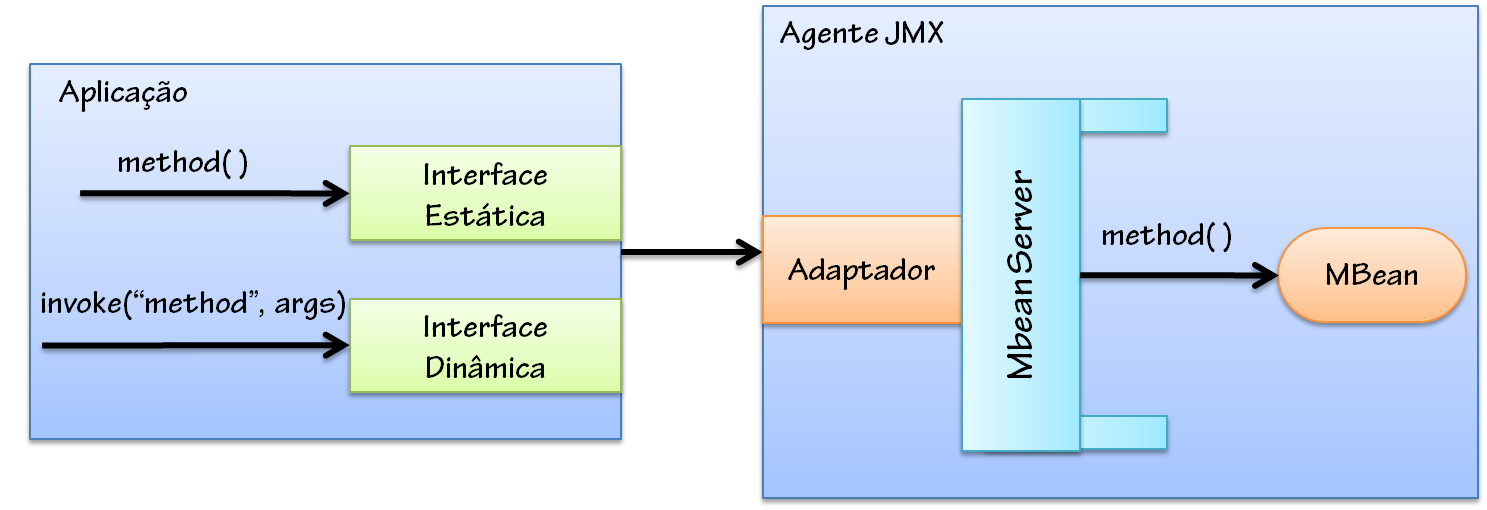
\includegraphics[width=13cm]{chapters/chapter4/invoke.png}
}
\\
\subfloat[Acesso a atributo na MBean]{
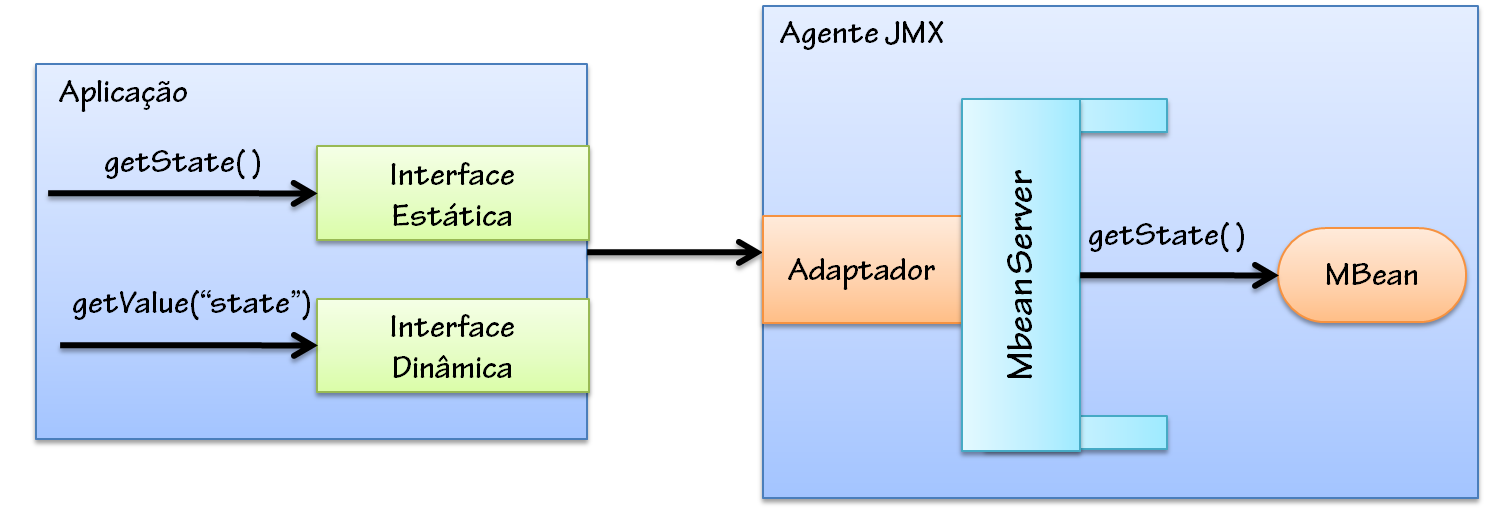
\includegraphics[width=13cm]{chapters/chapter4/getValue.png}
}
\caption{Acesso a atributos e operações da MBean.}
\label{fig:requestjmx}
\end{figure}

Exitem outros tipos de MBeans dinâmicas, como Model MBean, Open MBean e AbtractDynamicMBean que basicamente adicionam novas features à Dynamic MBean tradicional. Não entraremos em detalhes pois está fora do escopo deste trabalho.

\subsubsection{Nível Agente}
O nível agente é responsável por gerenciar todas as Mbeans e através delas controlar diretamente todos os recursos, tornando-os acessíveis a aplicativos de gerenciamento remoto.

A gerência das MBeans é provida através do principal componente do agente JMX, o MBean Server. Além disso, agentes JMX incluem um conjunto de serviços de gerenciamento de MBeans e pelo menos um adaptador de comunicações ou conector para permitir o acesso ao agente por aplicativos de gerenciamento~\cite{jmx}.

Basicamente, um agente JMX consiste em um MBean Server, um conjunto de serviços básicos de gerência e pelo menos um adaptador de comunicação ou conector JMX.

\paragraph{MBean Server:}
O MBean Server é o principal componente do nível agente. É o intermediário entre o sistema de gerenciamento e os objetos gerenciáveis (recursos), uma vez que, é responsabilidade do MBean Server registrar e manipular as MBeans~\cite{jmx}.

Para registrar uma MBean no servidor, além do próprio objeto MBean, é necessário que seja registrado junto a MBean um ObjectName que identifica unicamente aquela MBean no servidor. Além de identificar a MBean, ele permite a seleção de objetos a partir de mascaras no formato [domínio]:[par chave/valor]. \\
\verb org.meudominio:local=UFPE,nome=MBean \\

A manipulação de MBeans é feita através do MBean Server que provê um conjunto de operações comuns aos diferentes tipos de MBeans, uma vez que, os atributos e operações são descobertos através de classes de metadados comuns, ver parágrafo \ref{para:dynamicmbean}.

\subsubsection{Nível de Gerenciamento}
O nível de gerenciamento é o nível mais alto da arquitetura JMX, este define um mecanismo baseado em adaptadores e conectores que tornam os agente JMX acessíveis a aplicativos de gerenciamento remoto fora da JVM em que o agente encontra-se~\cite{jmx}.

Define, de certa forma, uma interface de acesso a agentes JMX para o mundo externo, através de protocolos proprietários ou existentes (\textit{e.g.} SNMP - \textit{Simple Network Manager Protocol}, um protocolo padrão para gerenciamento de componentes de rede)~\cite{douglas2005essential}.

Essa interface é garantida através de conectores e adaptadores que disponibilizam o acesos aos agentes JMX para diferentes tecnologia de gerenciamento.

A principal diferença entre conectores e adaptadores é que adaptadores surgem como uma solução de integração a sistemas que não dão suporte direto a JMX, por exemplo, sistemas de gerenciamento baseados em SNMP ou HTTP como Zabbix~\cite{zabbix} ou Nagios~\cite{nagios}, fornecendo uma visão de todos os MBeans através de um determinado protocolo. 

Já conectores, fornecem uma interface de gerenciamento remoto transparente e independente de protocolo~\cite{jmx}.


\subsection{Mecanismo Notificações}
Além dos três níveis de arquitetura, JMX provê um mecanismo de notificação que permite que aplicações ou MBeans recebam eventos ou notificações com informações sobre o estado dos recursos gerenciados, podendo gerar estatísticas ou mesmo processar eventos relacionados ao funcionamento dos recursos~\cite{lindfors2002jmx}.

O modelo de notificação JMX é semelhante ao mecanismo de notificações de java, que define \textit{object listers} (recebem as notificações) registados a MBean que envia as notificações \textit{(broadcaster MBeans)}. A \textit{broadcaster MBeans} envia eventos de notificação a todos os \textit{listeners} registrados~\cite{lindfors2002jmx}.

\subsubsection{Componentes do Mecanismo de Notificações}

O mecanismo de notificações JMX possui os seguintes componentes:

\begin{center}
\begin{table*}[h]
\begin{supertabular}[]{|l|l|}
\hline
\textbf{Componente} & \textbf{Descrição}\\\hline
Notification & Representa um tipo genérico de notificação\\\hline
NotificationListener & Interface que permite o recebimento de notificações\\\hline
\multirow{2}{*}{NotificationFilter} & Interface que permite a filtragem de notificações. Assim, apenas\\ 
& notificações relevantes ao Listener são recebidas\\\hline
\multirow{2}{*}{NotificationBroradcaster} & Interface que permite que notificações sejam enviadas aos\\
& listeners registrados \\\hline
\end{supertabular}
\caption{Componentes do Mecanismo de Notificação}
\end{table*}
\end{center}

\subsubsection{Modelo de Notificação JMX}
O modelo de notificações JMX segue os seguintes passos, demonstrados na Figura \ref{fig:notifyjmx}

\paragraph{Funcionamento} 
\begin{enumerate}
\item MBean consumidor registra-se através da interface \textit{NotificationBroadcaster}

\item MBean gerador emite uma notificação

\item A notificação é enviada aos MBeans registrados

\item O MBean consumidor recebe e filtra as notificações

\item As notificações não descartadas são tratadas
\end{enumerate}

\begin{figure}[h]
\centering
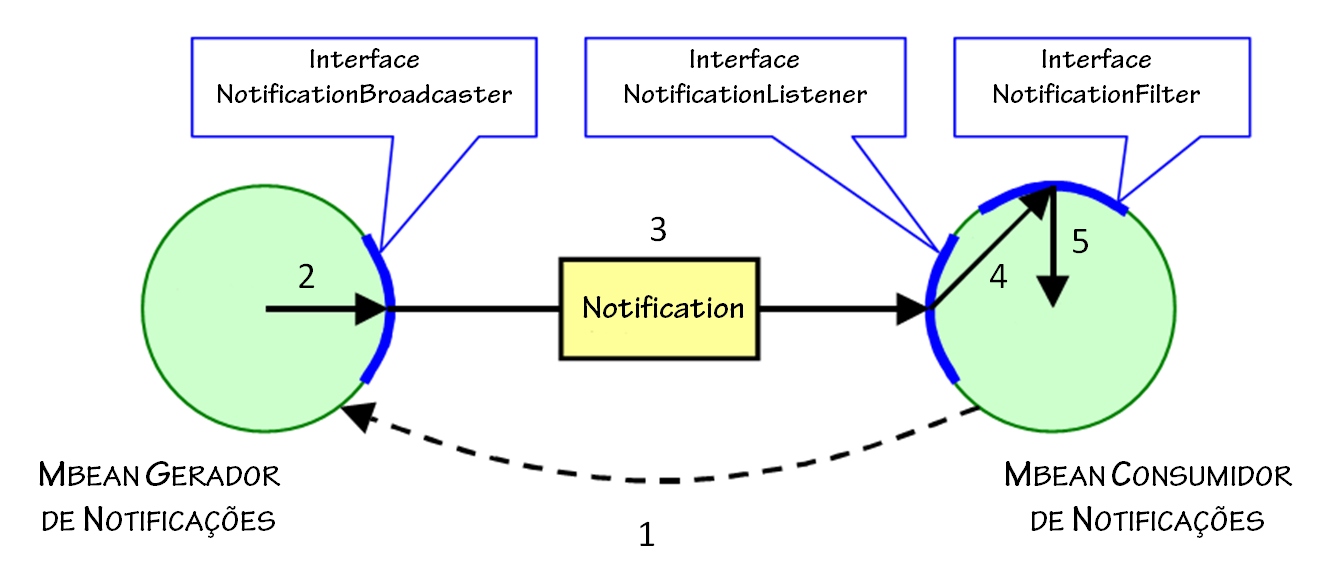
\includegraphics[width=13cm]{chapters/chapter4/notification_model.png}
\caption[Modelo de notificação JMX]{Modelo de notificação JMX.}
\label{fig:notifyjmx}
\end{figure}

TODO: fechar JMX